%\documentclass{article}
\documentclass[10pt,conference,compsocconf]{IEEEtran}

\newenvironment{proof}{\par \noindent {\bf Proof:}}{\begin{flushright}$\Box$\end{flushright}\par \noindent}
\newtheorem{theorem}{\bf Theorem}
\newtheorem{definition}[theorem]{\bf Definition}
\newtheorem{lemma}{\bf Lemma}
\newtheorem{corollary}[theorem]{\bf Corollary}
\newcommand{\pari}{\hspace{\parindent}}

\usepackage{amsmath}
\usepackage{latexsym}
\usepackage{amssymb}
\usepackage{listings}
\usepackage{tikz}
\usepackage{pdfpages}
\usepackage{cite}


\begin{document}

\title{Weekly Project Progress Report IV}

\author{\IEEEauthorblockN{Teng Yu%\IEEEauthorrefmark{1}
\IEEEauthorblockA{%\IEEEauthorrefmark{1}
}25th June 2016
}}
\date{}
\maketitle

\section{Achieved this week}

\begin{itemize}
%  \item Update the background report under Dr. Stillwell's advise. Discuss the difference between Allocation and Scheduling.
  \item Continue to implement the prototype architecture.  (API between reader and allocator) 
  \item Read the thesis \cite{van2015design}, focus on evaluation methods. Consider the targeting workloads are business-critical instead of focusing on scientific computing, so we are more interested in achieving high-availability against high-performance.
  \item Construct the initial partial-order model for the Business-critical workloads. Based on the statistical information as shown in  \cite{shen2015statistical} and computed from the trace directly (such as the maximum values for each dimension), we use "unit" instead of initial metrics for each dimension of resources to construct the model: Each unit for CPU and memory need equals to 2 CPU cores and 4GB memory, each unit for disk or network throughputs equals to 2MB/s.  
We only show the initial part of this model in Figure \ref{fig:f7} as the whole graph will be too complicate to present in here.  
    \item Apply the downsets representation and design ranking on the initial partial order model. As shown in Figure \ref{fig:f8}, we only give the initial part of the whole ranking system based on the same reason as above. The ranking value for each node in here is equal to the number of elements in each corresponding downsets. For easy illustration, we use $c_{\delta_{1}}d_{\delta_{2}}n_{\delta_{3}}$ to represent a record in the workload who needs $\delta_{1}$ units of CPU and memory, $\delta_{2}$ units of disk and $\delta_{3}$ units of network. The ranking value can be computed as following:
$$ Rank(\delta_{1},\delta_{2},\delta_{3})=\prod_{i=0}^{3}(\delta_{i}+1)-1 $$
  \item Do some theoretical analyse about the difference and advantage of our downset-representation approach against the traditional sum-of-vector method. Easy examples have been built to prove that downset representation can present the difference of resource capacities for different resource need even when the  sum of coordinates are equivalence between them.  As the sum-of-vector method is commonly used for heuristics, this analysis is meaningful for the evaluation design of this project.

\begin{figure}
\centering
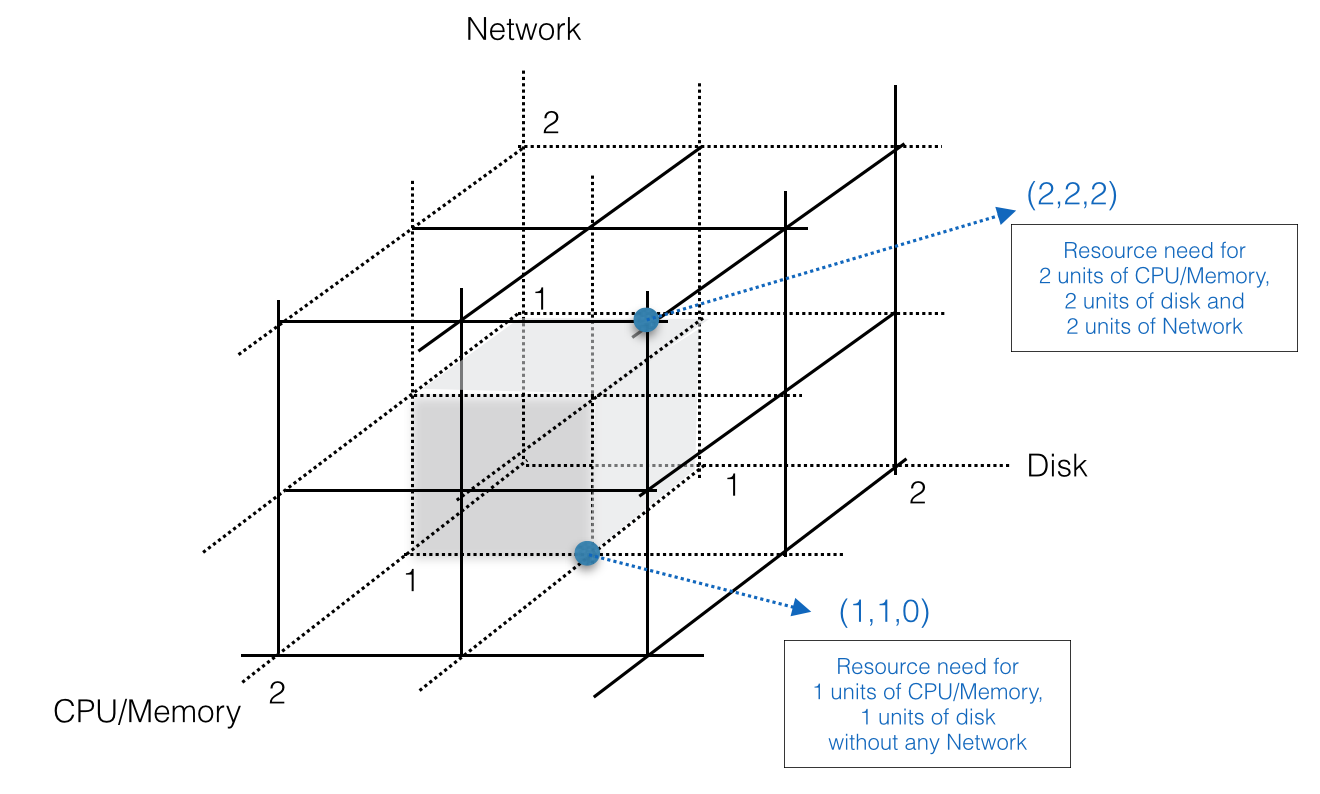
\includegraphics[scale=0.35]{InP.png}
\caption{Initial partial-order model for Business-critical workload}
\label{fig:f7}
\end{figure} 


\begin{figure}
\centering
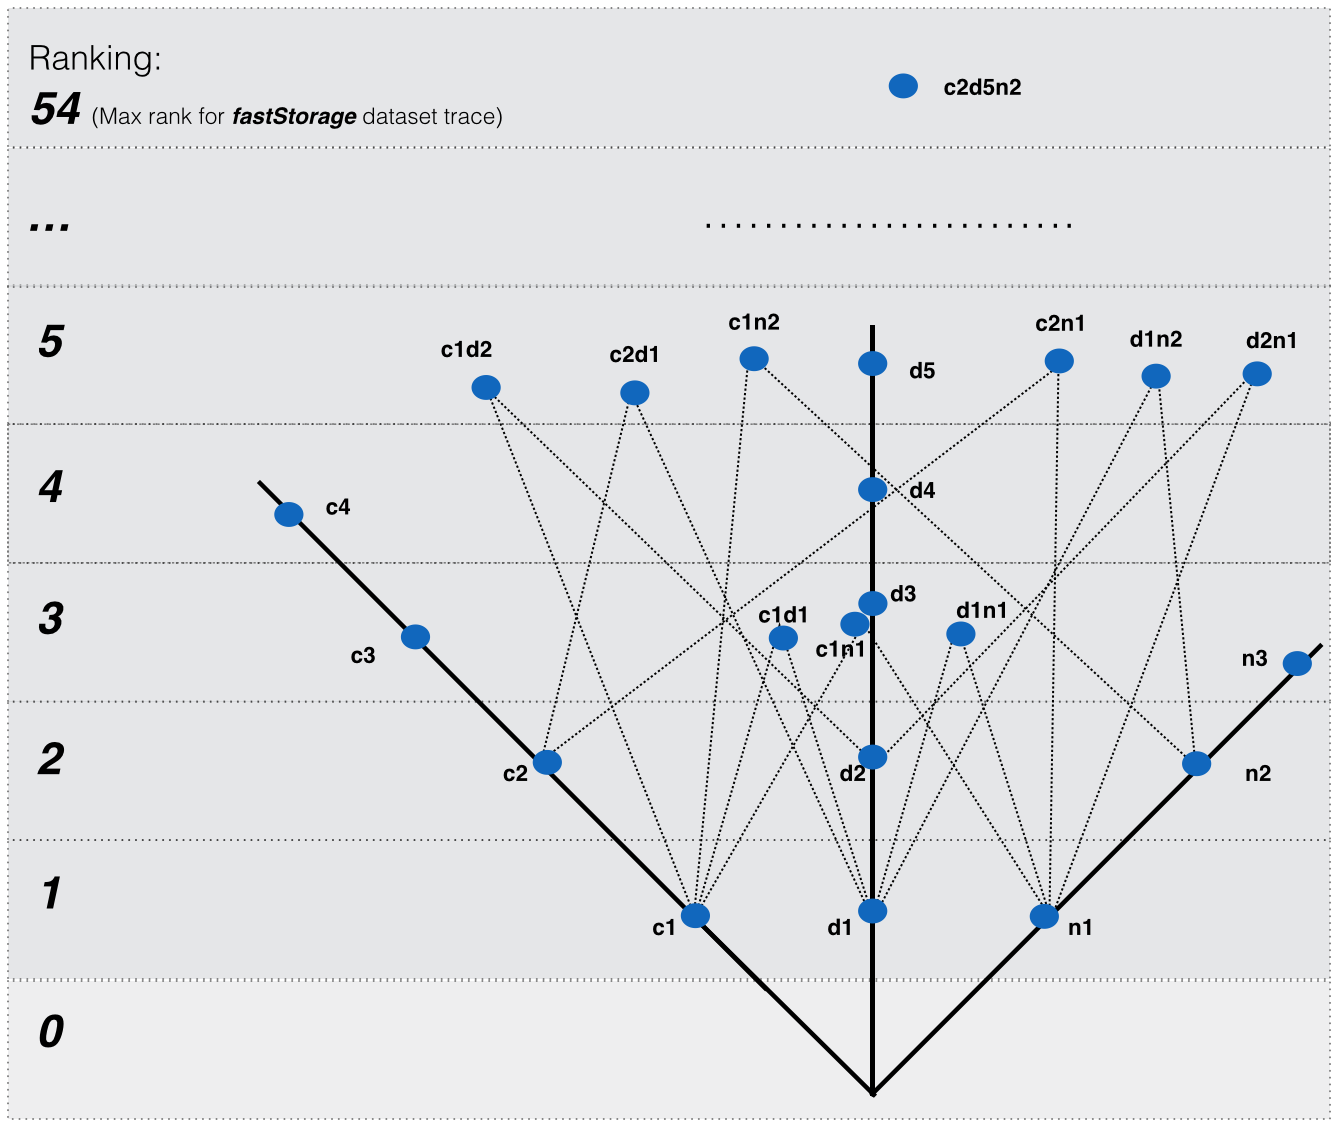
\includegraphics[scale=0.25]{InR.png}
\caption{Ranking model for Business-critical workload}
\label{fig:f8}
\end{figure} 
\end{itemize}


\section{Plan}
\begin{itemize}
  \item Further read the thesis \cite{van2015design}, focus on metrics and results.   
  \item Once the ranking values have been computed, I can begin to design the corresponding heuristic-based algorithms;
  \item Once the algorithms has been implemented, then the whole Rnrar architecture will be constructed targeting on business-critical workloads and general Cloud datacenters;
  \item The final step is evaluating our architecture on the workloads in \cite{shen2015statistical} based on the same simulation environment as in \cite{van2015self} and comparing the performance with their results as detailed presented in \cite{van2015design}.
\end{itemize}


\bibliographystyle{abbrv}
\bibliography{biblio}



\end{document}










Please refer to Fig. \ref{fig:f1}. for the proposed time table of the period: Thu. 2 - Thu. 7, Seven days. Feel free to change the date for the {\it whole-day-reserve} when needed for relaxation.
\begin{figure}
\centering
\includegraphics[scale=0.25]{tx1.png}
\caption{First Review Period}
\label{fig:f1}
\end{figure}



Please refer to Fig. \ref{fig:f2}. for the proposed time table of the period: Wed. 8 - Mon. 13.
\begin{figure}
\centering
\includegraphics[scale=0.25]{tx2.png}
\caption{Second Review Period}
\label{fig:f2}
\end{figure}



Please refer to Fig. \ref{fig:f3}. and Fig. \ref{fig:f4}. for the proposed time table of exams period. Please confirm the location and length of each exam.
\begin{figure}
\centering
\includegraphics[scale=0.20]{tx3.png}
\caption{First Exams Period}
\label{fig:f3}
\end{figure}

\begin{figure}
\centering
\includegraphics[scale=0.20]{tx4.png}
\caption{Final Exam}
\label{fig:f4}
\end{figure}
